\chapter{Crop a quarter of the image (center crop)}

\section{Idea}
\noindent
\begin{itemize}
    \item Calculate the new \texttt{top}, \texttt{bottom}, \texttt{left}, \texttt{right} positions after cropping the image using the following formulas:
\end{itemize}

\begin{center}
    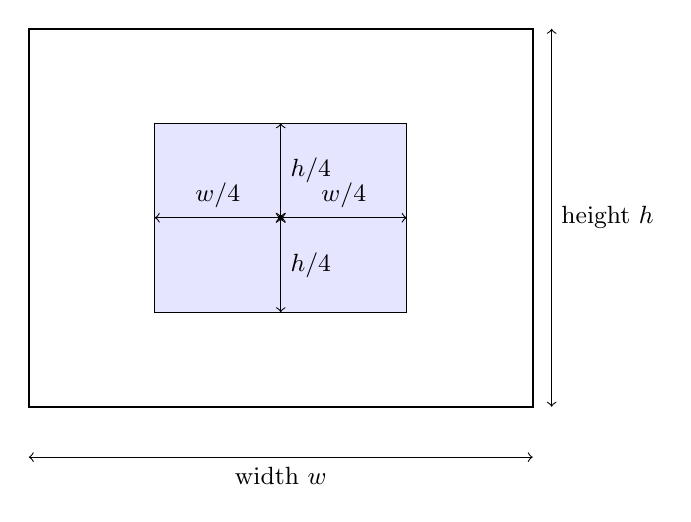
\begin{tikzpicture}[scale=0.8]
      \draw[thick] (0,0) rectangle (8,6);
    
      \draw[fill=blue!10] (2,1.5) rectangle (6,4.5);
    
      \filldraw[black] (4,3) circle (1pt);
    
      \draw[<->, black] (4,3) -- (2,3) node[midway, above] {\small $w/4$};
      \draw[<->, black] (4,3) -- (6,3) node[midway, above] {\small $w/4$};
    
      \draw[<->, black] (4,3) -- (4,1.5) node[midway, right] {\small $h/4$};
      \draw[<->, black] (4,3) -- (4,4.5) node[midway, right] {\small $h/4$};
    
      \draw[<->] (0,-0.8) -- (8,-0.8) node[midway, below] {\small width $w$};
      \draw[<->] (8.3,0) -- (8.3,6) node[midway, right] {\small height $h$};
    \end{tikzpicture}
\end{center}

\begin{itemize}
    \item The cropping process includes:
    \begin{itemize}[label=$\circ$]
        \item Starting from the center of the original image, the new top and bottom boundaries are defined by moving $\frac{h}{4}$ pixels up and down, respectively.
        \item Similarly, the new left and right boundaries are determined by moving $\frac{w}{4}$ pixels to the left and right from the center.
        \item The cropped image is obtained by extracting all pixels within the resulting rectangular region, bounded by these new top, bottom, left, and right positions.
    \end{itemize}
\end{itemize}

\section{Processing}
\begin{enumerate}
    \item Convert image to \texttt{float32} to avoid overflow during the process.
    \item Get the width and the height of the 2D image.
    \item Calculate the distance $\frac{h}{4}$ and $\frac{w}{4}$ from the center point of the image, which is used to determine new top/bottom and left/right position.
    \item Cropped image is obtained by collecting all pixels within the calculated position.
    \item Convert to \texttt{uint8} for correct display.
\end{enumerate}

\section{Result}
\begin{itemize}
    \item Original image/Cropped image
    \begin{center}
        \includegraphics[width=0.3\textwidth]{images/img.png}
        \includegraphics[width=0.3\textwidth]{images/img_quarter_crop.png}
    \end{center} 
    \begin{center}
        \includegraphics[width=0.3\textwidth]{images/img2.jpg}
        \includegraphics[width=0.3\textwidth]{images/img2_quarter_crop.jpg}
    \end{center} 
    \begin{center}
        \includegraphics[width=0.3\textwidth]{images/img3.jpg}
        \includegraphics[width=0.3\textwidth]{images/img3_quarter_crop.jpg}
    \end{center} 
\end{itemize}